% Mayuresh Vrushabhanath Pachore Thesis 2025-2026

% ===============================
% Document Class
% ===============================
\documentclass[12pt,a4paper,twoside]{book}

% ===============================
% Encoding & Language
% ===============================
\usepackage[T1]{fontenc}
\usepackage[utf8]{inputenc}
\usepackage[english]{babel}

% ===============================
% Page Layout
% ===============================
\usepackage{geometry}
\geometry{
    left=25mm,
    right=25mm,
    top=25mm,
    bottom=25mm
}

\usepackage{setspace}
\onehalfspacing % or \doublespacing if required

\usepackage{indentfirst}
\usepackage{pdflscape}

% ===============================
% Fonts
% ===============================
\usepackage{lmodern}        % Improved Computer Modern
\usepackage{microtype}      % Better typography

% ===============================
% Mathematics
% ===============================
\usepackage{amsmath}
\usepackage{amssymb}
\usepackage{amsfonts}
\usepackage{amsthm}
\usepackage{bm}             % Bold math symbols
\usepackage{mathtools}

% ===============================
% Graphics & Figures
% ===============================
\usepackage{graphicx}
\usepackage{float}
\usepackage{subcaption}
\usepackage{caption}
\usepackage{tikz}
\usetikzlibrary{arrows.meta,positioning,calc}

% ===============================
% Tables
% ===============================
\usepackage{booktabs}
\usepackage{multirow}
\usepackage{array}
\usepackage{longtable}
\usepackage{tabularx}

% ===============================
% Algorithms & Code
% ===============================
\usepackage{algorithm}
\usepackage{algpseudocode}

\usepackage{listings}
\usepackage{xcolor}

\lstset{
    basicstyle=\ttfamily\small,
    keywordstyle=\color{blue},
    commentstyle=\color{gray},
    stringstyle=\color{red},
    numbers=left,
    numberstyle=\tiny,
    frame=single,
    breaklines=true
}

% ===============================
% Units & Symbols
% ===============================
\usepackage{siunitx}
\sisetup{
    per-mode=symbol,
    detect-all
}

% ===============================
% Hyperlinks
% ===============================
\usepackage{hyperref}
\hypersetup{
    colorlinks=true,
    linkcolor=blue,
    citecolor=blue,
    urlcolor=blue
}


% ===============================
% Chapter/Section appearance  (PUT THIS HERE)
% ===============================
\usepackage{titlesec}

% Chapters: small "Chapter X", big title, better spacing
\titleformat{\chapter}[display]
  {\normalfont\bfseries}
  {\Large\chaptername\ \thechapter}
  {5ex}
  {\huge}



% ===============================
% Headings & TOC
% ===============================
\usepackage{chngcntr} % for \counterwithin
\usepackage{tocloft}
\usepackage{fancyhdr}
\pagestyle{fancy}
\fancyhf{}

% -----------------------
% Marks (chapter/section)
% -----------------------
\renewcommand{\chaptermark}[1]{\markboth{\thechapter.\ #1}{}}
\renewcommand{\sectionmark}[1]{\markright{\thesection.\ #1}}

% -----------------------
% Header
% -----------------------
% Left: current chapter/section
\fancyhead[L]{\small\nouppercase{\leftmark}}

% Right: page number (2.1, 2.2 ...)
\fancyhead[R]{\small\thepage}

% -----------------------
% Footer
% -----------------------

% Odd pages -> thesis title on left
\fancyfoot[L]{%
\ifodd\value{page}
\footnotesize \textit{\ThesisTitle}
\fi
}

% Even pages -> course/university on right
\fancyfoot[R]{%
\ifodd\value{page}
\else
\footnotesize \CourseUniversity
\fi
}

% -----------------------
% Lines
% -----------------------
\renewcommand{\headrulewidth}{0.4pt}
\renewcommand{\footrulewidth}{0.4pt}

% -----------------------
% First page of chapters
% -----------------------
\fancypagestyle{plain}{
\fancyhf{}
\fancyfoot[C]{\thepage}
\renewcommand{\headrulewidth}{0pt}
\renewcommand{\footrulewidth}{0pt}
}

% -----------------------
% Unnumbered chapters
% -----------------------
\fancypagestyle{chapterstar}{
\fancyhf{}
\fancyfoot[C]{\thepage}

\renewcommand{\headrulewidth}{0pt}
\renewcommand{\footrulewidth}{0pt}
}

\fancypagestyle{chapterplain}{
\fancyhf{}
\fancyfoot[L]{\footnotesize \CourseUniversity}
\fancyfoot[R]{\footnotesize \thepage}
\renewcommand{\headrulewidth}{0pt}
\renewcommand{\footrulewidth}{0.4pt}
}

\fancypagestyle{chapternum}{
  \fancyhf{}

  % Header
  \fancyhead[L]{\small\rightmark}
  \fancyhead[R]{\small\thepage}

  % Footer
  \fancyfoot[R]{%
    \ifodd\value{page}
      \footnotesize \textit{\ThesisTitle}
    \fi
  }

  \fancyfoot[L]{%
    \ifodd\value{page}
    \else
      \footnotesize \CourseUniversity
    \fi
  }

  \renewcommand{\headrulewidth}{0.4pt}
  \renewcommand{\footrulewidth}{0.4pt}
}


% ===============================
% Appendices
% ===============================
\usepackage{appendix}

% ===============================
% Nomenclature / Acronyms
% ===============================
\usepackage{nomencl}
\makenomenclature

% \usepackage[acronym]{glossaries}
% \makeglossaries

% ===============================
% PDF Inclusion
% ===============================
\usepackage{pdfpages}

% ===============================
% Line Breaking & Widow Control
% ===============================
\usepackage[all]{nowidow}

% ===============================
% Custom Commands (optional)
% ===============================
\newcommand{\R}{\mathbb{R}}
\newcommand{\vect}[1]{\boldsymbol{#1}}

\newcommand{\AuthorName}{\textit{Manuel Mo}}
\newcommand{\ThesisTitle}{Italian Named Entity Recognition with Transformer Models: A Comparative Evaluation of UmBERTo and XLM-RoBERTa on the NERMuD 2023 Benchmark}
\newcommand{\CourseUniversity}{Natural Language Processing, Computer Science, University of Bologna}

\newcommand{\origcleardoublepage}{}

\setlength{\headheight}{14pt}

% ===============================
% End of Preamble
% ===============================


\begin{document}

    %Only for title page 
    \setlength{\parindent}{15pt}
    \setlength{\parskip}{15mm}
    
    \begin{titlepage}
        \begin{center}
            
\includegraphics[width=6.5cm,height=4.7cm]{figs/Unibo_Logo.png}

            {\large{\bf{Second Dycle Degree Programme in Computer Science (6698) - Natural Language Processing (91258)}}}

        
            {\bfseries\fontsize{26pt}{20pt}\selectfont
                \setlength{\lineskip}{2pt}%
                \setlength{\lineskiplimit}{0pt}%
                Italian Named Entity Recognition with Transformer Models\par}
                
            {\large{\bf{A Comparative Evaluation of UmBERTo and XLM-RoBERTa on the NERMuD 2023 Benchmark}}}

        \end{center}
        
        \begin{minipage}[t]{0.5\textwidth}
            {\Large{\bf Professor: \\ Fabio Tamburini}}
            \vspace{6mm}

            
        \end{minipage}
        \hfill
        \begin{minipage}[t]{0.40\textwidth}\raggedleft
            {\Large{\bf Student: \\ Manuel Mo}}
        \end{minipage}

        \rule[0.5mm]{15.3845cm}{0.4mm}
        \vspace{-\baselineskip}
        \begin{center}
            {\large\bfseries October 21 of 2026\\}
            {\large\bfseries Academic Year 2026/2027}
        \end{center}

    \end{titlepage}

    \pagenumbering{roman} %page numbering is roman letters for this section
    \setlength{\parindent}{15pt}
    \setlength{\parskip}{0pt}
    
	\chapter*{Abstract}
    \addcontentsline{toc}{chapter}{Abstract}
    \thispagestyle{chapterstar}
	\label{abstract_Eng}
	This report presents the fine-tuning and evaluation of two pretrained Transformer models, UmBERTo and XLM-RoBERTa, for Named Entity Recognition (NER) using the NERMuD 2023 dataset. The study compared an Italian-specific model with a multilingual model to investigate their performance on Italian named entity recognition.

FALTA FALAR QUE É DO CURSO NLP O NOME DO PROF ETC
	\clearpage
	
	%table of contents
    \tableofcontents
    \thispagestyle{chapterstar}
    \clearpage
    \pagestyle{fancy}

    \addcontentsline{toc}{chapter}{List of Figures}
	\listoffigures
    \thispagestyle{chapterstar}
	\clearpage

    \listoftables
    \thispagestyle{chapterstar}
    \addcontentsline{toc}{chapter}{List of Tables}
    \clearpage

    \let\origcleardoublepage\cleardoublepage
    \let\cleardoublepage\clearpage
    \chapter*{Acronyms}
    \addcontentsline{toc}{chapter}{Acronyms}
    \thispagestyle{chapterstar}
	\label{Acronyms}
	\begin{table}[h!]
\centering
\begin{tabular}{p{3cm} p{11cm}}
\hline
\textbf{Symbol} & \textbf{Description} \\
\hline

ADG & Alcide De Gasperi \\
API & Application Programming Interface \\
BERT & Bidirectional Encoder Representations from Transformers \\
BIO & Beginning, Inside, Outside \\
BLSTM & Bidirectional Long Short-Term Memory \\
CRF & Conditional Random Field \\
DAC & Domain-Agnostic Classification \\
DSC & Domain-Specific Classification \\
EVALITA & Evaluation of NLP and Speech Tools for Italian \\
FIC & Fiction \\
GPU & Graphics Processing Unit \\
IOB & Inside-Outside-Beginning \\
JSONL & JavaScript Object Notation Lines \\
LOC & Location \\
NER & Named Entity Recognition \\
NERMuD & Named-Entities Recognition on Multi-Domain Documents \\
NLP & Natural Language Processing \\
ORG & Organization \\
PER & Person \\
RNN & Recurrent Neural Network \\
WN & Wikinews \\
WWM & Whole Word Masking \\
XLM-R & Cross-lingual RoBERTa \\

\hline
\end{tabular}
\end{table}

    \mainmatter 
    \pagestyle{chapternum}
    
    \pagenumbering{arabic}
    \counterwithin{page}{chapter}
    \renewcommand{\thepage}{\thechapter.\arabic{page}}
    
	\chapter{Introduction}
    \thispagestyle{chapterplain}
	\label{chap:introduction}
	%=============================================================
% CHAPTER 1: INTRODUCTION
%=============================================================

Named Entity Recognition (NER) is a fundamental task in Natural Language Processing (NLP) that involves identifying and classifying named entities in text, such as persons, organizations, and locations \cite{mohit2014ner}. By extracting structured information from unstructured texts, NER facilitates the identification of relevant information and supports a wide range of NLP applications, including information extraction, document classification, and question answering. It is particularly useful for processing large volumes of textual data, allowing relevant entities to be identified more efficiently.

Recent advances in NLP have been driven by Transformer-based models, which have demonstrated strong performance across a wide range of language understanding tasks \cite{vaswani2017attention}. Pretrained language models can be fine-tuned on annotated datasets to adapt their representations to specific tasks, including NER. However, model performance may vary depending on the language and the characteristics of the text being processed.

This project investigates the performance of two pretrained Transformer models on Italian NER: UmBERTo, a model pretrained specifically for Italian, and XLM-RoBERTa, a multilingual model trained on text from multiple languages. The experiments use the NERMuD 2023 dataset, which covers three distinct domains: news, fiction, and political speeches. This dataset provides an opportunity to evaluate the models across different types of Italian text.

The main goal is to compare the performance of these two models under comparable experimental conditions and investigate whether language-specific pretraining provides an advantage over multilingual pretraining for Italian NER. Both models are fine-tuned on the same training data and evaluated using the same evaluation procedure.

The remainder of this report is organized as follows. Chapter 1 presents relevant background and related work. Chapter 2 describes the dataset and experimental methodology. Chapter 3 presents the experimental results followed by a discussion. Finally, Chapter 4 summarizes the main conclusions.

%-------------------------------------------------------------
\section{Background and Related work}
\label{sec:background}
%-------------------------------------------------------------

\subsection{Named Entity Recognition}
\label{subsec:ner}

Named Entity Recognition (NER) is an NLP task that consists of identifying and classifying named entities in text into predefined categories \cite{mohit2014ner}. Common entity categories include persons, organizations, and locations.

For example, consider the following sentence: ``The operation for Pope Leo will take place at the Agostino Gemelli Polyclinic Hospital in Rome.'' A NER system could identify \textit{Pope Leo} as a person, \textit{Agostino Gemelli Polyclinic Hospital} as an organization, and \textit{Rome} as a location. This process transforms unstructured text into structured information that can be used by other NLP applications.

NER is useful in a variety of applications, including information extraction, question answering, machine translation, and document analysis. By automatically identifying relevant entities, NER systems can facilitate the retrieval and organization of information from large collections of text.

However, identifying named entities can be challenging because the same word may refer to different entities depending on its context, and entities may consist of multiple words. These challenges make NER an important task in NLP research.

\subsection{Transformer-based Language Models}
\label{subsec:transformer}

Before the introduction of Transformers, recurrent neural networks (RNNs), particularly Bidirectional Long Short-Term Memory networks (BLSTMs) combined with Conditional Random Fields (CRFs), were widely used for sequence labeling tasks such as Named Entity Recognition. The introduction of the Transformer architecture marked a significant development in NLP, enabling models to capture contextual relationships between words through a mechanism known as self-attention \cite{vaswani2017attention}.

Unlike recurrent architectures, which process sequences step by step, Transformers can process tokens in parallel during training and model relationships between tokens regardless of their distance in a sequence. This allows them to learn contextual representations that are useful for a wide range of language understanding tasks.

The development of pretrained Transformer-based language models, such as BERT, further advanced NLP by enabling models to learn general linguistic representations from large text collections. These models can then be fine-tuned on task-specific annotated datasets, adapting their learned representations to tasks such as NER \cite{devlin2019bert}.

This approach is particularly relevant to the present study, which investigates whether an Italian-specific pretrained model, UmBERTo, achieves better NER performance than the multilingual XLM-RoBERTa model. Both models are based on Transformer architectures and can be fine-tuned for token-level classification.


\subsection{umBERTo and XLM-RoBERTa}
\label{subsec:berts}

UmBERTo and XLM-RoBERTa are pretrained language models based on the Transformer architecture, but they differ in their pretraining data and language coverage.

UmBERTo is a RoBERTa-based language model specifically developed for Italian. The model used in this project, \texttt{umberto-commoncrawl-cased-v1}, was pretrained on a large Italian text corpus derived from OSCAR, which is based on Common Crawl data. It uses SentencePiece tokenization and Whole Word Masking, an approach in which entire words are masked during pretraining rather than individual subword tokens \cite{musixmatch2020umberto}.

In contrast, XLM-RoBERTa (XLM-R) is a multilingual language model pretrained on text from 100 languages using a large collection of filtered Common Crawl data. It follows a masked language modelling objective, learning contextual representations by predicting masked tokens. Its multilingual pretraining allows it to represent text in different languages within a shared model \cite{conneau2020xlmr}.

These differences make the two models suitable for comparison in Italian Named Entity Recognition. UmBERTo benefits from pretraining focused specifically on Italian, whereas XLM-RoBERTa learns representations from a multilingual corpus. Comparing their performance on the same dataset can help investigate whether language-specific pretraining provides an advantage for this task.

\subsection{NERMuD 2023}
\label{subsec:nermud}

NERMuD (Named-Entities Recognition on Multi-Domain Documents) was a shared task organized as part of the EVALITA 2023 evaluation campaign for Italian Natural Language Processing. Its objective was to evaluate named entity recognition systems on documents from different domains, focusing on three entity categories: persons, organizations, and locations \cite{palmeroaprosio2023nermud}.

The task covered three domains: news, fiction, and political speeches. It included two subtasks: Domain-Agnostic Classification (DAC), which required a single model to process documents from all three domains, and Domain-Specific Classification (DSC), which allowed a separate model to be developed for each domain \cite{palmeroaprosio2023nermud}.

In this project, the NERMuD 2023 dataset is used to fine-tune and evaluate UmBERTo and XLM-RoBERTa. By considering documents from different domains, the experiments investigate how the two models perform on Italian text beyond a single type of document. The comparison uses the same dataset splits and evaluation procedure for both models to support a fair assessment of their performance.

    \let\cleardoublepage\origcleardoublepage

	\clearpage{\pagestyle{empty}\cleardoublepage}
		
			
    \chapter{Dataset and Methodology}
    \thispagestyle{chapterplain}
    \label{chap:dataset-method}
	
\section{The dataset}
\label{sec:dataset}

FALTA FALAR DO TIPO DE FICHEIRO E MOSTRAR UM EXEMPLO DE UMA FRASE

The experiments in this project use the NERMuD 2023 dataset, developed as part of the EVALITA 2023 evaluation campaign for Italian Natural Language Processing. The dataset focuses on Named Entity Recognition across different types of Italian text, covering three entity categories: persons, organizations, and locations \cite{palmeroaprosio2023nermud}.

The dataset contains documents from three domains: Wikinews (WN), fiction (FIC), and writings and speeches by Alcide De Gasperi (ADG). These domains represent different writing styles and contexts, providing a basis for evaluating NER systems across different types of text.

Wikinews contains journalistic texts, fiction consists of excerpts from Italian literary works, and the ADG domain contains political writings and speeches. These differences are relevant to NER because the frequency, distribution, and context of named entities may vary between domains.

\subsection{Dataset Organization}
\label{subsec:data-org}

The NERMuD 2023 dataset is organized into multiple files according to their domain and purpose. Each domain is divided into training, development, and test subsets. In this project, the corresponding subsets from the three domains are combined to create a single training set, a single development set, and a single test set. The domain information is retained to support further analysis of model performance across domains.

Table~\ref{tab:dataset-splits} presents the number of examples in each subset.

\begin{table}[htbp]
    \centering
    \caption{Number of examples in each NERMuD 2023 data split.}
    \label{tab:dataset-splits}
    \begin{tabular}{lrrr}
        \hline
        \textbf{Domain} & \textbf{Train} & \textbf{Dev} & \textbf{Test} \\
        \hline
        Wikinews (WN) & 10,912 & 2,594 & 2,088 \\
        Fiction (FIC) & 11,423 & 1,051 & 1,517 \\
        Alcide De Gasperi (ADG) & 5,147 & 1,122 & 521 \\
        \hline
        \textbf{Total} & \textbf{27,482} & \textbf{4,767} & \textbf{4,126} \\
        \hline
    \end{tabular}
\end{table}

The training set is used to fine-tune the models, while the development set is used to monitor their performance during training and select the best model checkpoint. The test set is reserved for the final evaluation, allowing the performance of both models to be compared on data that was not used for training or model selection.

\subsection{Entity Categories and Annotation Scheme}
\label{subsec:ent-cat}

The dataset contains three named entity categories: persons (PER), organizations (ORG), and locations (LOC). These categories identify people, institutions or other organizations, and geographical places, respectively.

The original annotations follow the Inside-Outside-Beginning (IOB) tagging scheme, commonly referred to as BIO. In this scheme, each token receives a label indicating whether it belongs to a named entity and, if so, whether it begins the entity or continues it. The labels used in this project are:

\begin{itemize}
\item \texttt{B-PER}, \texttt{B-ORG}, and \texttt{B-LOC}: the first token of a person, organization, or location entity.
\item \texttt{I-PER}, \texttt{I-ORG}, and \texttt{I-LOC}: subsequent tokens belonging to the corresponding entity.
\item \texttt{O}: a token that does not belong to any named entity.
\end{itemize}

For example, the sentence ``Umberto Guidoni visited Rome'' can be annotated as follows:

\begin{table}[htbp]
    \centering
    \caption{Example of BIO annotation.}
    \label{tab}
    \begin{tabular}{ll}
        \hline
        \textbf{Token} & \textbf{Label} \\
        \hline
        Umberto & B-PER \\
        Guidoni & I-PER \\
        visited & O \\
        Rome & B-LOC \\
        \hline
    \end{tabular}
\end{table}

This representation allows the models to perform token-level classification while preserving information about the boundaries and categories of named entities.


\section{Data Preprocessing}
\label{sec:preprocessing}

Before training, the dataset is processed to ensure that the text tokens and their corresponding entity labels are correctly aligned. The original annotations are converted into a consistent representation containing the text tokens, their BIO labels, and their domain.

The preprocessing procedure includes tokenizing the text, locating the annotated entities, and assigning the appropriate BIO labels to the corresponding tokens. Particular attention is given to multi-word entities, whose first token receives a beginning label and whose subsequent tokens receive continuation labels.

Whitespace and punctuation differences can make it difficult to match annotated entity strings exactly to their occurrences in the original text. To address these cases, normalized matching is used as a fallback when an exact match cannot be found. This procedure helps align the annotations without unnecessarily modifying the original text.

After preprocessing, the resulting data is stored in a structured format for use in the subsequent training and evaluation stages. The same processed dataset splits are used for both models to maintain consistency in the experimental setup.

\section{Experimental Setup}
\label{sec:experimental-setup}

Two pretrained Transformer-based language models are evaluated: UmBERTo and XLM-RoBERTa. Both models are fine-tuned for token-level classification using the BIO labels described above.

The experiments use the same training, development, and test splits. The development set is used to monitor performance and select the best checkpoint, whereas the test set is reserved for the final comparison. Keeping the data splits and evaluation procedure consistent helps ensure that differences in performance can be compared meaningfully.

The following chapter presents the experimental results and discusses the performance of the two models.


	\clearpage{\pagestyle{empty}\cleardoublepage}
	

    \chapter{Results and Discussion}
    \thispagestyle{chapterplain}
    \label{chap:methodology}
	\section{Exploratory Data Analysis}
\label{sec:eda}

An exploratory data analysis was performed to characterize the NERMuD 2023 dataset beyond the basic split counts presented in Section~\ref{sec:dataset}. The analysis focuses on three aspects that are relevant for interpreting model performance: the imbalance between domains, the distribution of entity types, and the length of the input sequences.

\subsection{Domain Imbalance}
\label{subsec:eda-domain}

As shown in Table~\ref{tab:dataset-splits}, the three domains are not equally represented. Wikinews and fiction contain substantially more samples than the ADG domain, both in training and in test data. This imbalance is relevant when interpreting model performance: results on the smaller ADG domain may be influenced by the lower number of training examples, and a model that performs well on WN and FIC is not necessarily equally effective on ADG.

\subsection{Entity Distribution}
\label{subsec:eda-entities}

The dataset contains three entity types: persons (PER), organizations (ORG), and locations (LOC). Figure~\ref{fig:entity-distribution} presents the number of entities of each type across the splits. Person entities are the most frequent in the training set, followed by locations and organizations, and all three categories are represented in substantial numbers. The distribution is reasonably consistent across splits, ensuring that all entity types are represented in the development and test sets.

\begin{figure}[H]
    \centering
    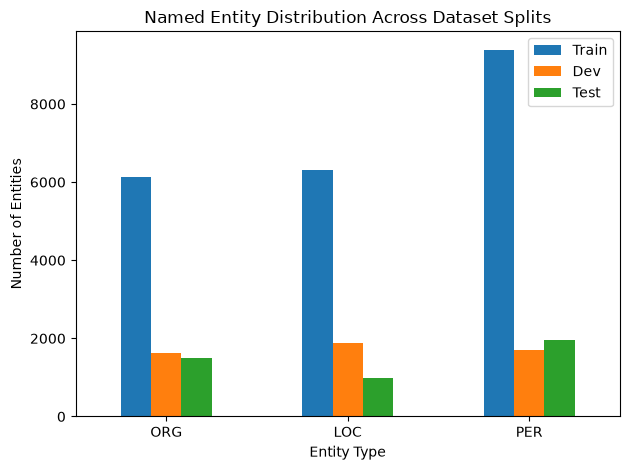
\includegraphics[width=0.65\textwidth]{figs/entity_distribution.png}
    \caption{Distribution of named entity types across dataset splits.}
    \label{fig:entity-distribution}
\end{figure}

The distribution of entity types also varies considerably across domains, as shown in Table~\ref{tab:entity-domain} for the training set. The FIC domain contains a notably high number of person entities but relatively few organization entities, whereas WN presents a more balanced distribution and the largest number of entities overall. These differences suggest that the domains place different demands on the models: a model trained mostly on fiction may be less exposed to organization entities, while a model trained on news may see a broader range of entity types.

\begin{table}[H]
    \centering
    \caption{Named entity distribution across domains in the training set.}
    \label{tab:entity-domain}
    \begin{tabular}{lrrr}
        \hline
        \textbf{Domain} & \textbf{LOC} & \textbf{ORG} & \textbf{PER} \\
        \hline
        ADG & 915  & 1,531 & 889 \\
        FIC & 587  & 137   & 3,177 \\
        WN  & 4,800 & 4,454 & 5,325 \\
        \hline
    \end{tabular}
\end{table}

\subsection{Sequence Length}
\label{subsec:eda-length}

The length of the input sequences was analyzed to determine an appropriate maximum sequence length for the experiments. Table~\ref{tab:sequence-length} presents descriptive statistics for the three splits.

\begin{table}[H]
    \centering
    \caption{Sequence length statistics in tokens.}
    \label{tab:sequence-length}
    \begin{tabular}{lrrr}
        \hline
        \textbf{Statistic} & \textbf{Train} & \textbf{Dev} & \textbf{Test} \\
        \hline
        Count  & 27,482 & 4,767 & 4,126 \\
        Mean   & 20.46 & 23.43 & 24.45 \\
        Std.   & 15.78 & 16.45 & 17.83 \\
        Min.   & 1 & 1 & 1 \\
        Median & 17 & 20 & 21 \\
        Max.   & 251 & 130 & 137 \\
        \hline
    \end{tabular}
\end{table}

Figure~\ref{fig:text-length} illustrates the distribution of sequence lengths. Most sequences are relatively short, with the majority concentrated well below the maximum observed length. The maximum length in the training set is 251 tokens, while the development and test sets reach 130 and 137 tokens, respectively. Based on these observations, a maximum sequence length of 256 tokens was selected for the Transformer models, providing sufficient capacity for the observed sequences while limiting unnecessary padding during training.

\begin{figure}[H]
    \centering
    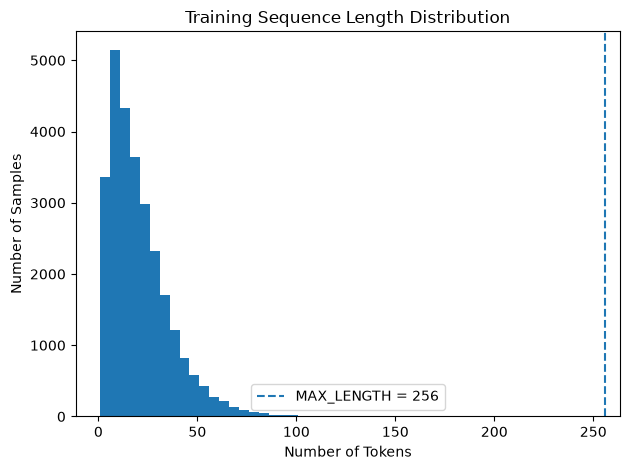
\includegraphics[width=0.7\textwidth]{figs/text_length_distribution.png}
    \caption{Distribution of sequence lengths in the NERMuD 2023 dataset.}
    \label{fig:text-length}
\end{figure}

\section{Model Training}
\label{sec:train}

Both models were fine-tuned for token-level classification using the Hugging Face \texttt{Transformers} library \cite{wolf2020transformers}. The training procedure was kept as similar as possible between the two models, so that differences in performance can be attributed mainly to the pretrained representations rather than to the training setup.

\subsection{Training Configuration}
\label{subsec:train-config}

The same hyperparameters were used for both models, including the effective batch size. Table~\ref{tab:train-config} summarizes the configuration, and the paragraphs below explain the rationale behind each choice.

\begin{table}[H]
    \centering
    \caption{Training configuration for UmBERTo and XLM-RoBERTa.}
    \label{tab:train-config}
    \begin{tabular}{lll}
        \hline
        \textbf{Parameter} & \textbf{UmBERTo} & \textbf{XLM-RoBERTa} \\
        \hline
        Max sequence length & 256 & 256 \\
        Learning rate & $2 \times 10^{-5}$ & $2 \times 10^{-5}$ \\
        Per-device batch size & 8 & 1 \\
        Gradient accumulation & -- & 8 \\
        Effective batch size & 8 & 8 \\
        Epochs & 3 & 3 \\
        Weight decay & 0.01 & 0.01 \\
        Optimizer & AdamW & AdamW \\
        Mixed precision (fp16) & No & Yes \\
        Random seed & 42 & 42 \\
        \hline
    \end{tabular}
\end{table}

\textbf{Maximum sequence length.} A maximum sequence length of 256 tokens was selected based on the exploratory analysis in Section~\ref{subsec:eda-length}, which showed that virtually all sequences in the dataset fall below this limit. This value provides sufficient capacity for the observed sequences while limiting the amount of unnecessary padding during training.

\textbf{Learning rate and weight decay.} A learning rate of $2 \times 10^{-5}$ and a weight decay of 0.01 follow common practices for fine-tuning Transformer models on token-classification tasks \cite{devlin2019bert}. Smaller learning rates are typically used for fine-tuning than for training from scratch, because the pretrained weights already encode useful representations that should not be destroyed by large updates.

\textbf{Effective batch size.} Both models were trained with an effective batch size of 8. UmBERTo fits a per-device batch size of 8 directly in GPU memory. XLM-RoBERTa, however, has a much larger vocabulary (250,002 tokens, compared to 32,005 for UmBERTo), which increases the memory required for the embedding layer and the classifier. To keep the effective batch size comparable, XLM-RoBERTa was trained with a per-device batch size of 1 and gradient accumulation over 8 steps. This means that gradients are accumulated over 8 forward passes before each optimizer update, producing an update equivalent to a batch of 8 examples.

\textbf{Mixed precision.} Mixed-precision training (\texttt{fp16}) was enabled for XLM-RoBERTa to reduce memory usage and speed up training on GPU. For UmBERTo, \texttt{fp16} was left disabled, since the model trained comfortably with full precision and the smaller vocabulary did not require the additional memory savings.

\textbf{Number of epochs.} Three epochs were used for both models. This value was chosen as a compromise between underfitting (too few epochs) and overfitting (too many epochs on a relatively small dataset), and the development set was used to verify that no clear overfitting occurred.

\textbf{Optimizer.} The AdamW optimizer, which is the default in the Hugging Face \texttt{Trainer}, was used for both models. AdamW decouples weight decay from the gradient update, which generally leads to better generalization than standard Adam.

\textbf{Random seed.} The random seed was fixed to 42 at the beginning of each notebook, controlling weight initialization, data shuffling, and dropout, which improves the reproducibility of the experiments. The \texttt{data\_seed} argument was also set to 42 for XLM-RoBERTa to ensure that data shuffling is reproducible independently of the model seed.

\subsection{Training Dynamics}
\label{subsec:train-dynamics}

The development set was evaluated after every epoch, and the checkpoint with the highest development F1-score was retained for final evaluation. Table~\ref{tab:dev-f1} reports the development F1-score obtained by each model at the end of each epoch.

\begin{table}[H]
    \centering
    \caption{Development F1-score after each training epoch.}
    \label{tab:dev-f1}
    \begin{tabular}{lccc}
        \hline
        \textbf{Model} & \textbf{Epoch 1} & \textbf{Epoch 2} & \textbf{Epoch 3} \\
        \hline
        UmBERTo & 0.8602 & 0.8724 & \textbf{0.8834} \\
        XLM-RoBERTa & 0.8070 & 0.8359 & \textbf{0.8519} \\
        \hline
    \end{tabular}
\end{table}

Both models improved steadily across the three epochs, and the best development F1-score was obtained in the final epoch in both cases. This suggests that additional epochs could potentially yield further gains, although the improvement between the second and third epochs was already smaller than between the first and the second, indicating that the models were approaching convergence.

Training time differed substantially between the two models. UmBERTo completed three epochs in approximately 18 minutes, whereas XLM-RoBERTa required 1 hour and 11 minutes under the gradient-accumulation and mixed-precision setting described above. This difference reflects both the larger vocabulary of XLM-RoBERTa and the additional forward passes required by gradient accumulation.

The comparison between the two models is fair with respect to the optimization regime: both were trained with the same effective batch size (8), the same learning rate, the same number of epochs, the same data splits, and the same evaluation procedure. Gradient accumulation was used for XLM-RoBERTa so that its effective batch size matches that of UmBERTo, despite the smaller per-device batch size required by its larger vocabulary.

However, the comparison does not control for every possible factor. The two models differ not only in pretraining language coverage but also in tokenizer vocabulary, pretraining corpus, and pretraining objective. Part of the observed difference in performance may therefore be attributable to these factors rather than to the language coverage of the pretraining data alone. The results should be interpreted as a comparison between two specific pretrained checkpoints under a shared training protocol, rather than as a controlled experiment isolating the effect of language-specific pretraining.

\subsection{Implementation}
\label{subsec:train-impl}

Training was implemented using the Hugging Face \texttt{Trainer} API. The model, tokenizer, data collator, and evaluation metrics were configured through small utility modules (\texttt{config.py}, \texttt{data\_utils.py}, \texttt{metrics.py}, and \texttt{models\_utils.py}) so that both models are trained with the same code path.

Token-level labels were aligned with subword tokens using the standard \texttt{word\_ids} strategy: the first subword of each word receives the original BIO label, while the remaining subwords and special tokens are assigned the label \texttt{-100} and ignored by the loss function \cite{devlin2019bert}. This ensures that the model is trained on word-level entity boundaries rather than on arbitrary subword fragments.

\section{Model Evaluation}
\label{sec:eval}

\section{Discussion}
\label{sec:disc}


	\clearpage{\pagestyle{empty}\cleardoublepage}
	
    \chapter{Conclusion}
    \thispagestyle{chapterplain}
    \label{chap:conc}
	This project investigated the performance of two pretrained Transformer models on Italian Named Entity Recognition: UmBERTo, an Italian-specific model, and XLM-RoBERTa, a multilingual model. Both models were fine-tuned on the NERMuD 2023 dataset under comparable experimental conditions, with the same data splits, the same effective batch size, the same learning rate, and the same evaluation procedure.

The results show that UmBERTo outperforms XLM-RoBERTa on the test set, with a global F1-score of 0.8945 against 0.8743. The advantage of the Italian-specific model is consistent across all three entity types (PER, ORG, and LOC) and across two of the three domains (Wikinews and ADG). The only exception is the fiction domain, where XLM-RoBERTa obtains a slightly higher F1-score (0.8902 against 0.8828). These results suggest that language-specific pretraining provides an advantage for Italian NER, but that this advantage depends on the type of text being processed.

The analysis also identified several patterns that are consistent across both models. Person entities are the easiest category to predict, organizations are the hardest, and the ADG domain is the most difficult of the three domains. These patterns are consistent with the distribution of entity types and training examples in the dataset, and they highlight the importance of considering the characteristics of the target text when choosing a NER model.

\section{Future Work}
\label{sec:future-work}

Several directions for future work can be identified.

\textbf{Multiple runs and statistical testing.} Training each model with multiple random seeds and reporting the mean and standard deviation of the F1-score would allow the robustness of the observed differences to be assessed. Statistical significance testing (for example, a paired bootstrap test on the test set) would help determine whether the domain-level differences, in particular the advantage of XLM-RoBERTa on fiction, are meaningful.

\textbf{Additional checkpoints.} Comparing larger versions of the two models (for example, XLM-RoBERTa-large or other UmBERTo variants) would provide a more complete picture of the trade-off between language-specific and multilingual pretraining.

\textbf{Domain-specific fine-tuning.} Since the results suggest that the advantage of each model depends on the domain, a natural extension would be to fine-tune separate models for each domain (the DSC subtask of NERMuD 2023) and compare them with a single domain-agnostic model (the DAC subtask). This would show whether the domain-level differences observed here persist when the models are specialized.

\textbf{Other Italian datasets.} Evaluating the two models on other Italian NER datasets would help determine whether the conclusions generalize beyond NERMuD 2023.

Overall, this project provides a controlled comparison between an Italian-specific and a multilingual Transformer for Italian NER, and shows that language-specific pretraining can provide a measurable advantage on this task, although the advantage is not uniform across domains. These findings contribute to a better understanding of when language-specific pretraining is worth the additional effort of training or selecting a dedicated model, and when a multilingual model may be sufficient.
	\clearpage{}
		
    % \chapter{Experimental Setup}
    % \thispagestyle{chapterplain}
    % \label{chap:experimental-setup}
	% This project investigated the performance of two pretrained Transformer models on Italian Named Entity Recognition: UmBERTo, an Italian-specific model, and XLM-RoBERTa, a multilingual model. Both models were fine-tuned on the NERMuD 2023 dataset under comparable experimental conditions, with the same data splits, the same effective batch size, the same learning rate, and the same evaluation procedure.

The results show that UmBERTo outperforms XLM-RoBERTa on the test set, with a global F1-score of 0.8945 against 0.8743. The advantage of the Italian-specific model is consistent across all three entity types (PER, ORG, and LOC) and across two of the three domains (Wikinews and ADG). The only exception is the fiction domain, where XLM-RoBERTa obtains a slightly higher F1-score (0.8902 against 0.8828). These results suggest that language-specific pretraining provides an advantage for Italian NER, but that this advantage depends on the type of text being processed.

The analysis also identified several patterns that are consistent across both models. Person entities are the easiest category to predict, organizations are the hardest, and the ADG domain is the most difficult of the three domains. These patterns are consistent with the distribution of entity types and training examples in the dataset, and they highlight the importance of considering the characteristics of the target text when choosing a NER model.

\section{Future Work}
\label{sec:future-work}

Several directions for future work can be identified.

\textbf{Multiple runs and statistical testing.} Training each model with multiple random seeds and reporting the mean and standard deviation of the F1-score would allow the robustness of the observed differences to be assessed. Statistical significance testing (for example, a paired bootstrap test on the test set) would help determine whether the domain-level differences, in particular the advantage of XLM-RoBERTa on fiction, are meaningful.

\textbf{Additional checkpoints.} Comparing larger versions of the two models (for example, XLM-RoBERTa-large or other UmBERTo variants) would provide a more complete picture of the trade-off between language-specific and multilingual pretraining.

\textbf{Domain-specific fine-tuning.} Since the results suggest that the advantage of each model depends on the domain, a natural extension would be to fine-tune separate models for each domain (the DSC subtask of NERMuD 2023) and compare them with a single domain-agnostic model (the DAC subtask). This would show whether the domain-level differences observed here persist when the models are specialized.

\textbf{Other Italian datasets.} Evaluating the two models on other Italian NER datasets would help determine whether the conclusions generalize beyond NERMuD 2023.

Overall, this project provides a controlled comparison between an Italian-specific and a multilingual Transformer for Italian NER, and shows that language-specific pretraining can provide a measurable advantage on this task, although the advantage is not uniform across domains. These findings contribute to a better understanding of when language-specific pretraining is worth the additional effort of training or selecting a dedicated model, and when a multilingual model may be sufficient.
	% \clearpage{\pagestyle{empty}\cleardoublepage}
	
	
    % \chapter{Results and Discussion}
    % \thispagestyle{chapterplain}
    % \label{chap:results}
	% \section{Quantitative Results}
\label{sec:quantitative-results}

    \subsection{Comparison with Baselines}
    \label{subsec:baseline-comparison}

    \subsection{Performance Across Datasets}
    \label{subsec:dataset-performance}

\section{Qualitative Analysis}
\label{sec:qualitative-analysis}

    \subsection{Case Studies}
    \label{subsec:case-studies}

    \subsection{Visual Inspection of Outputs}
    \label{subsec:visual-inspection}

\section{Ablation Study}
\label{sec:ablation}

    \subsection{Impact of Each Component}
    \label{subsec:component-impact}

    \subsection{Sensitivity Analysis}
    \label{subsec:sensitivity}

\section{Discussion}
\label{sec:discussion}

    \subsection{Interpretation of Results}
    \label{subsec:interpretation}

    \subsection{Limitations of the Proposed Method}
    \label{subsec:limitations}


4h 3min 16sec
	% \clearpage{\pagestyle{empty}\cleardoublepage}

    	
    \pagestyle{plain}
    \setcounter{page}{1}
    \renewcommand{\thepage}{B\arabic{page}}
    \bibliographystyle{ieeetr}
    \addcontentsline{toc}{chapter}{Bibliography}
    \bibliography{references}

\end{document}

